\documentclass[12pt]{report}

% ok, prometto che la prossima volta dividerò in sottodocumenti

\usepackage[italian]{babel}
\usepackage[latin1]{inputenc}
\usepackage{url}
\usepackage{biblatex}
\usepackage{amsmath}
\usepackage{graphicx}
\usepackage{caption}
\usepackage{float}
\usepackage{array}
\usepackage[margin=2cm]{geometry}
\usepackage{changepage}
\usepackage{color}
\usepackage{multirow}


\hyphenation{ransac}
	
%\bibliography{bib}

\begin{titlepage}
\begin{adjustwidth}{}{-3.7cm}
\begin{center}

\\[2.1cm]

\textsc{\Large Progetto di \\ Image Analysis and Synthesis \\ e \\ Argomenti avanzati di analisi di immagini}\\[0.5cm]
\textsc{\large A.A. 2010/2011}\\[0.5cm]

% Title
\\[1.5cm]
{ \huge \bfseries iaasFog}\\[0.4cm]
{ \huge \bfseries Analisi della visibilit\'a in \\ condizioni di nebbia}\\[0.4cm]
\\[1.5cm]

% Author and supervisor
\begin{minipage}{0.8\textwidth}
\begin{flushleft} \large
Stefano \textsc{Cadario},\\ mat. 724842\\
Luca \textsc{Cavazzana},\\ mat. 734498
\end{flushleft}
\end{minipage}
\begin{minipage}{0.8\textwidth}
\begin{flushright} \large
Prof.~Vincenzo \textsc{Caglioti}
\end{flushright}
\end{minipage}

%\vfill
\\[4cm]

% Bottom of the page
{\large 17 maggio 2011}

\end{center}
\end{adjustwidth}
\end{titlepage}


\begin{document}
%\maketitle

\tableofcontents

\chapter{Introduzione}

L'obbiettivo del progetto \`e estrarre un parametro numerico indicante la visibilit\`a in caso di nebbia utilizzando esclusivamente delle immagini riprese da una telecamera montata su un'automobile. La tecnica utilizzata si basa sull'analisi della variazione del contrasto delle features individuate in ogni frame dell'immagine con il fine di trovare il parametro $\lambda$ della funzione

$$k_fe^{-t_{imp}/\lambda}$$

\noindent Tale funzione deriva da una prima analisi teorica del problema in questione: la variabile $t_{imp}$ rappresenta il tempo che occorre ad una feature per attraversare il piano immagine, $k_f$ \`e il massimo livello di contasto di una generica feature $f$ in condizioni di visibilit\'a ideali, mentre il parametro $\lambda$, globale, pu\`o essere visto come il tempo d'impatto per una feature che sta emergendo dalla nebbia prendendo come riferimento l'istante in cui il livello di contrasto assume il valore $k_f/e$.\\
\noindent Il livello di visibilit\`a, che \`e una distanza, dovr\`a poi essere calcolato considerando la velocit\`a del veicolo come $\lambda v_t$.\\

\noindent I problemi affrontati nel corso di questo progetto consistono nello sviluppo di una tecnica performante per l'individuazione e il tracking di features il cui movimento relativo sia consistente con quello del veicolo, e trovare un metodo per il calcolo del contrasto e per la stima dei parametri in questione sufficientemente robusto ai livelli di rumore sui dati.\\
	 	
\noindent Un simile sistema potrebbe essere integrato fra i sensori di un veicolo, monitorando l'idoneit\`a della velocit\`a di crociera rispetto alle condizioni di visibilit\`a e ai tempi di reazione del conducente. Nel campo emergente dei veicoli autonomi, similmente, potrebbe vincolare il valore massimo di velocit\`a in base ai tempi di risposta, oppure potenziare la consapevolezza del sistema di analisi d'immagine fornendo un parametro per la stima della qualit\`a dei dati a seconda della distanza dell'elemento da cui sono state ricavati.



\chapter{Implementazione}

\section{Tracking delle features}


\noindent Il tracking delle features\footnote{All'interno di questo documento con il termine ``feature'' ci si riferisce ad una sequenza di corner associati ad uno stesso dettaglio nella scena in frame successivi.} deve individuare il maggior numero di features in ogni immagine, e nel contempo escludere gli outliers che influirebbero nei passaggi successivi dell'elaborazione.\\
L'analisi dei frame avviene in modo inverso rispetto al tempo, in modo da individuare le features quando sono ben visibili per poi inseguirle nei frame temporalmente precedenti, dove il riconoscimento \`e pi\`u difficoltoso a causa della nebbia.\\

\noindent Ad ogni frame viene eseguita la funzione \verb|cvGoodFeaturesToTrack| che individua la posizione dei corner con autovalori pi\`u alti e quindi con maggior probabilit\`a di essere individuati nei frame successivi. Nel frame seguente vengono quindi inseguiti utilizzando la funzione \verb|cvCalcOpticalFlowPyrLK|, che utilizzando l'algoritmo iterativo di \emph{Lucas-Kanade} ricalcola la nuova posizione di ogni feature.\\

\noindent Prima di aggiungere alla sequenza il nuovo punto individuato vengono effettuati dei controlli di coerenza: la nuova posizione deve avere direzione concorde con i punti antecedenti ed il nuovo passo deve essere maggiore dei precedenti. Una sequenza di corner \`e considerata valida se \`e inseguita per almeno cinque frame (per ottenere una migliore approsimazione del birapporto), in caso contrario viene eliminata. Se la feature \`e valida viene eseguito un controllo sulla cross-ratio dei punti, che deve essere prossima a 4/3. I punti trovati saranno comunque soggetti ad errori di posizione dovuti a diversi fattori e quindi non collineari: per rimediare viene quindi calcolata la retta di regressione, su cui verranno proiettati i punti per l'analisi del birapporto.\\

\noindent Il tracking dei corner diventa sempre pi\`u difficoltoso all'avvicinarsi al vanishing point a causa del calo dei livelli di contrasto dovuti alla nebbia, che riduce la possibilit\`a di individuazione; per ovviare a questo problema vengono calcolate le posizioni teoriche delle features utilizzando i punti nei frame precedenti e la cross ratio nota. Il tracking di una feature ha termine quando non si hanno pi\`u frame disponibili oppure quando lo step del nuovo punto \`e inferiore a $0.5$ pixel.

\section{Calcolo del vanishing point}
La posizione del vanishing point riveste un ruolo fondamentale nella risoluzione del problema poich\'e viene coinvolto sia nel filtro degli outliers, sia nel calcolo del tempo d'impatto di ogni feature.\\

\noindent Inizialmente \`e stato implementato un algoritmo che prevedeva l'individuazione di tutti i punti di intersezione tra rette e da questi ricavare il punto che minimizza la distanza con tutti gli altri. Questo approccio, sebbene abbia dato buoni risultati, si \`e rivelato troppo lento a causa della complessit\`a eccessiva del problema che richiedeva fino a $15$ secondi di elaborazione per $200$ features (complessit\`a $O\left(n^4\right)$).\\

\noindent Dopo un primo tentativo di ottimizzare l'algoritmo gi\'a esistente si \`e deciso di tentare un approccio completamente nuovo sfruttando RANSAC:

\begin{itemize}
\item	Ad ogni iterazione viene eletto casualmente un possibile candidato vanishing point calcolando l'intersezione delle rette rappresentanti due features, con il solo vincolo di essere all'interno del field of view dell'immagine.
\item	Per ogni retta viene calcolata la distanza dal vanishing point candidato. Tali distanze vengono ordinate in un vettore, la cui mediana sar\`a il rank associata a quel particolare vanishing point.
\item	Se il nuovo vanishing point ha un rank migliore dei precedenti viene eletto come nuovo best vanishing point.
\item	Il ciclo termina quando vengono analizzati un numero di intersezioni ritenuto sufficiente (il $5\%$ di tutte le possibili intersezioni tra rette).
\end{itemize}

\noindent Vengono infine scartate le features la cui retta di regressione dista pi\`u della distanza mediana rispetto al vanishing point eletto in quanto probabili outliers (viene mantenuta quindi solo la met\'a delle features).

\begin{figure}
	\begin{minipage}[b]{0.5\linewidth}
		\centering
		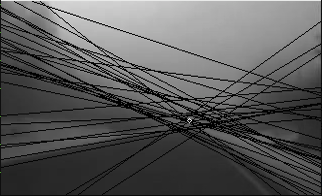
\includegraphics[scale=0.6]{images/iaasBefore.png}
		\captionof{figure}{Vanishing point calcolato mediante RANSAC.}
		\label{fig:vpBef}
	\end{minipage}
	\hspace{0.5cm}
	\begin{minipage}[b]{0.5\linewidth}
		\centering
		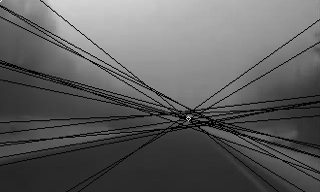
\includegraphics[scale=0.6]{images/iaasAfter.png}
		\captionof{figure}{Linee di fuga coerenti con il vanishing point calcolato.}
		\label{fig:vpAft}
	\end{minipage}


\end{figure}

\noindent L'algoritmo applicato a diversi set di dati ha restituito buoni risultati con tempi notevolmente ridotti (circa $1$ secondo di elaborazione per $200$ features) rispetto alla precedente implementazione meno efficiente (complessit\`a $O\left(n^2\log{n}\right)$).\\

\noindent Opzionalmente la posizione del vanishing point reale pu\`o essere affinata utilizzando SVD sul $50\%$ delle rette pi\`u vicine al vanishing point trovato in precedenza.\\

\begin{center}
	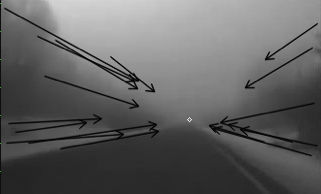
\includegraphics[scale=0.7]{images/iaasAfterArrow.png}
	\captionof{figure}{Flusso delle features inseguite.}
	\label{fig:vpAftArr}
\end{center}

\section{Calcolo del tempo all'impatto}

\noindent Dato un set di punti di coordinate $A$ e $B$ rappresentanti una feature in differenti immagini e conoscendo il frame rate $f$ delle telecamera \`e possibile calcolare il tempo d'impatto, ossia l'istante in cui la feature attraverser\`a il piano immagine, mediante il birapporto

$$ cross(i,a,b,v) = \frac{\overline{ia}}{\overline{ab}}\frac{\overline{av}}{\overline{iv}} = \frac{\overline{i'a'}}{\overline{a'b'}}\frac{\overline{a'v'}}{\overline{i'v'}} $$

\noindent dove $a$ e $b$ sono le coordinate delle feature, $v$ quelle del vanishing point e $i$ l'intersezione della traiettoria con il piano immagine, nel mondo reale e all'interno dei frames.\\
\noindent Essendo nel mondo reale le distanze rispetto al vanishing point infinite, cos\`i come quelle rispetto al piano della telecamera nelle immagini, la formula si semplifica in

$$ \frac{\overline{ia}}{\overline{ab}} = \frac{\overline{a'v'}}{\overline{a'b'}} $$

\noindent Dal momento che $\overline{a'v'}$ e $\overline{a'b'}$ sono noti, ed essendo $ab$ la distanza percorsa dal veicolo fra le due immagini ($velocit\`a/frame rate$), il tempo d'impatto pu\`o essere ottenuto come

$$ t_{i} = \frac{\overline{a'v'}}{\overline{a'b'}}\frac{\overline{ab}}{v} = \frac{\overline{a'v'}}{\overline{a'b'}}f^{-1} $$

\section{Calcolo del contrasto}

\noindent Per il calcolo del contrasto nell'intorno delle features sono stati presi in considerazione diversi approcci: oltre alla formule di Michelson e Weber, gi\`a sfruttate nelle precedenti fasi del progetto, \`e stato deciso di introdurre anche Root Mean Square, che calcola il livello di contrasto secondo la formula

$$ c\left(I_{M\times N}\right) = \sqrt{\frac{1}{MN}\sum_{i=1}^N\sum_{j=1}^M(i_{ij}-\bar{I})^2} $$

\noindent Dal momento che nel calcolo del valore contribuiscono tutti i pixel all'interno della finestra tale formula risulta essere molto pi\`u resistente al rumore rispetto alle precendenti, il cui risultato risulta essere influenzato dall'errore sul singolo pixel centrale per Weber, e dall'errore sui valori di min e max per Michelson.\\

\noindent Confrontando i valori ottenuti calcolando i livelli di contrasto utilizzando i diversi metodi si nota come RMS tenda a generare curve pi\`u smooth (figure \ref{fig:contr01}, \ref{fig:contr02} e \ref{fig:contr03}).\\

\noindent Una particolarit\`a di RMS \`e che, al contrario delle altre tecniche, il risultato dipende dallo spazio di colori utilizzato per rappresentare l'immagine (facilmente risolvibile riscalando rispetto alla profondit\`a del colore).

\begin{center}
	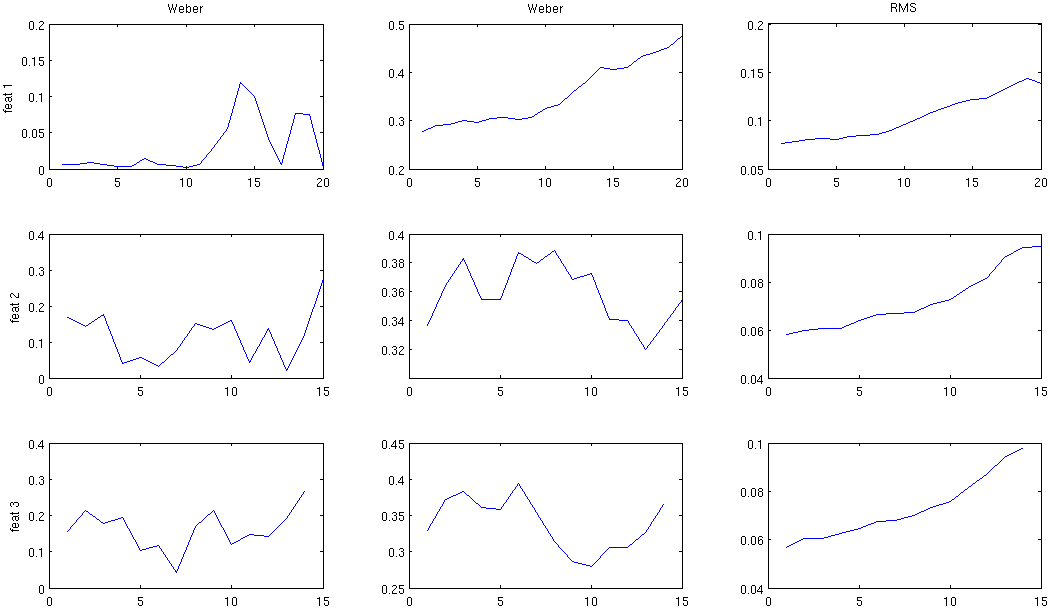
\includegraphics[scale=0.7, angle=90.0]{images/compContr1.png}
	\captionof{figure}{confronto fra i valori di contrasto ottenuti mediante i differenti approcci.}
	\label{fig:contr01}
\end{center}
\begin{center}
	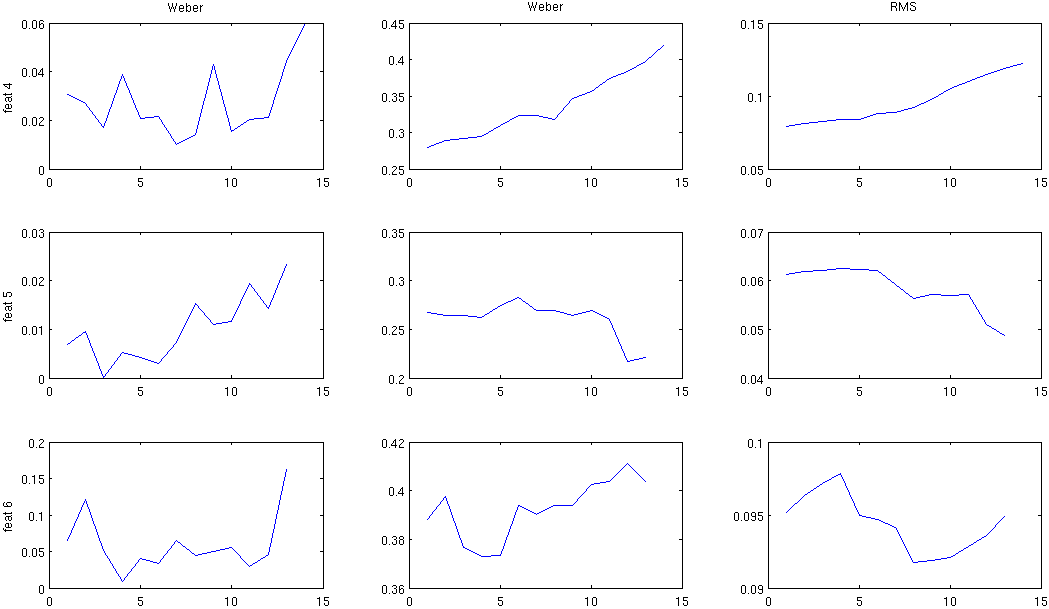
\includegraphics[scale=0.7, angle=90.0]{images/compContr2.png}
	\captionof{figure}{confronto su nuove features.}
	\label{fig:contr02}
\end{center}
\begin{center}
	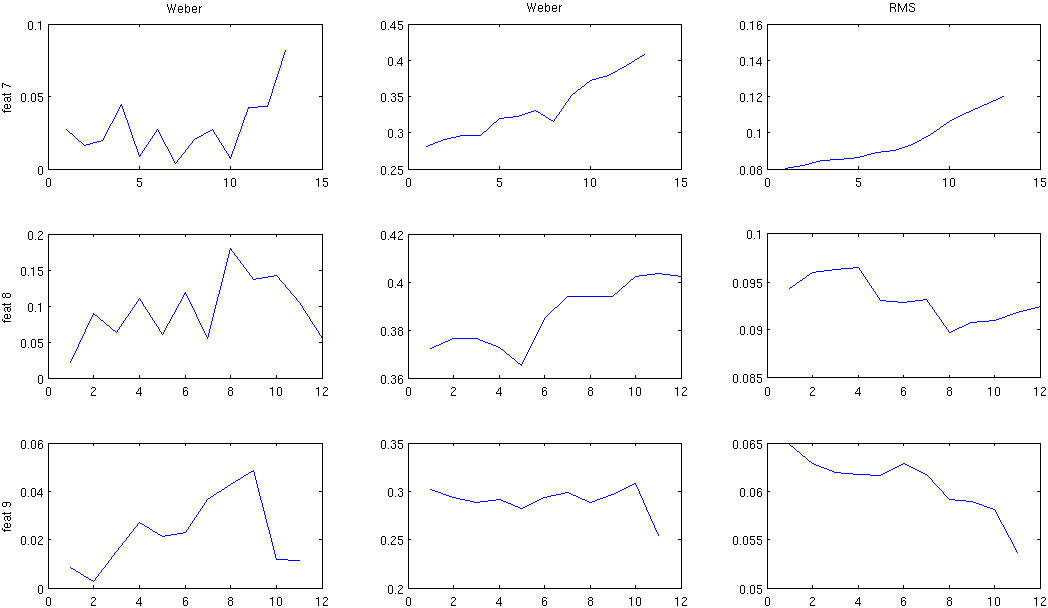
\includegraphics[scale=0.7, angle=90.0]{images/compContr3.png}
	\captionof{figure}{confronto su nuove features.}
	\label{fig:contr03}
\end{center}




\section{Stima dei parametri}

\noindent La visibilit\`a viene espressa come una distanza: tale misura potrebbe essere calcolata mediante il birapporto note le posizioni di un certo numero di landmark presenti nella scena o mediante il tempo all'impatto data la velocit\`a del veicolo. Sfortunatamente tali informazioni per il video campione fornito non sono disponibili, quindi ci si \`e limitati a considerare il tempo d'impatto medio calcolato per il parametro $\lambda$ come valutazione delle condizioni di visibilit\`a nell'ipotesi (forte) di velocit\`a costante.\\

\subsection{Fitting di $\lambda$}

\noindent Una prima tecnica adottata \`e stata quella di sfruttare la funzione \verb|fit| di Matlab per estrarre il parametri $k_f$ e $\lambda_f$ che meglio descrivono ogni singola feature mediante il metodo dei minimi quadrati non lineare. Per ogni dato viene cos\`i calcolato l'errore rispetto alla curva generata, valore in base al quale verr\'a selezionata la met\'a dei dati migliori che verranno riutilizzati per approssimare nuovamente i parametri di una seconda curva esponenziale.\\

\begin{center}
	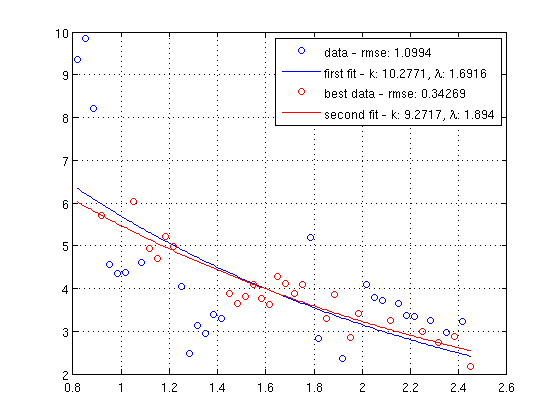
\includegraphics[scale=0.7]{images/twoFits.png}
	\captionof{figure}{Due fitting consecutivi: il blu usando tutta la sequenza di contrasti, in rosso la curva ottenuta usando solo il $50\%$ dei dati con errore migliore.}
	\label{fig:twoFits}
\end{center}

\noindent Fra i nuovi $\lambda_f$ calcolati vengono selezionati quelli associati al quartile delle migliori curve (meno affette da rumore), scelte in base ad un valore calcolato mediante diversi approcci:

\begin{itemize}
	\item	\emph{errore primo/secondo fitting}: l'errore viene calcolato come media dei rapporti fra l'errore e la proiezione del dato sulla prima/seconda curva approssimante calcolata.
	\item	\emph{variazione dell'errore}: nell'ipotesi di un buon set di dati la variazione dell'errore medio non dovrebbe essere molto grande. Viene quindi tenuta in considerazione la differenza fra gli errori dei dati sulle due curve (prossima a $0$ per buone features) o il loro rapporto (prossimo a $1$).
	\item	\emph{errore integrale}: sempre nell'ipotesi che per un buon set di dati la variazione fra le due curve \`e minima, viene calcolata la variazione sui parametri. Per aggregare i due valori viene considerata la differenza fra l'area delle due curve, calcolata come $$\left|\int^{\infty}_0\left(k_1e^{-t_{imp}/\lambda_1} - k_2e^{-t_{imp}/\lambda_2}\right)dt\right| =$$ $$= \left|\left[ k_2\lambda_2e^{-t_{imp}/\lambda_2} - k_1\lambda_1e^{-t_{imp}/\lambda_1} \right]^\infty_0\right| =$$ $$ = \left|k_2\lambda_2 - k_1\lambda_1\right|$$
\end{itemize}

\noindent L'ultimo approccio appare essere quello pi\`u robusto, ed \`e quello selezionato di default nel codice. Il $\lambda$ globale viene cos\`i calcolato come la mediana di quelli delle features selezionate.

\subsection{Normalizzazione mediante fitting di $k$ e RANSAC}

\noindent Un'altra tecnica sperimentata consiste nel calcolare il parametro $k_f$ della curva che minimizza l'errore su ogni singola feature.\\

\begin{figure}[H]
	\centering
	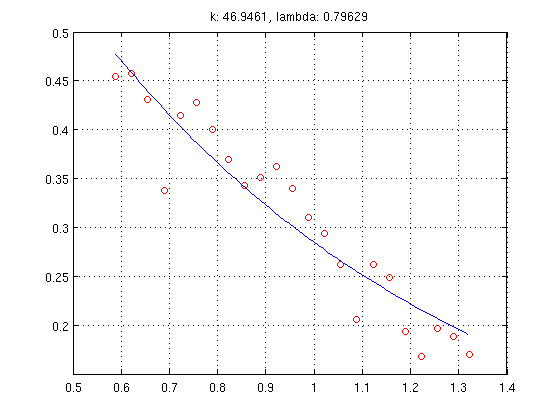
\includegraphics[scale=0.6]{images/fitting.png}
	\captionof{figure}{Fitting e rescaling di una singola feature.}
	\label{fig:fitting}
\end{figure}

\noindent Tale parametro viene utilizzato per normalizzare features con differenti valori di contrasto ``intrinseco'' (ovvero il massimo livello che otterremmo in condizioni ideali, senza nebbia): utilizzando $c_{i,f}/k_f$ possiamo cos\`i considerare sulla funzione discreta solo il contributo della nebbia, permettendoci di aggregare i contrasti di diverse features e stimare il parametro $\lambda$ globale sulla formula $ c\left(t_{imp}\right) = e^{-t_{imp}/\lambda} $ mediante RANSAC.\\

\noindent Questa implementazione di RANSAC seleziona a caso il $25\%$ dei set disponibili: i valori di contrasto vengono aggregati, ordinati in base al tempo d'impatto ed infine usati per stimare il $\lambda$ globale usando il parametro della curva approssimante. Per tale parametro verr\`a poi calcolato il set di consenso ed il relativo errore, iterando il processo come da manuale.\\

\begin{figure}[H]
	\centering
	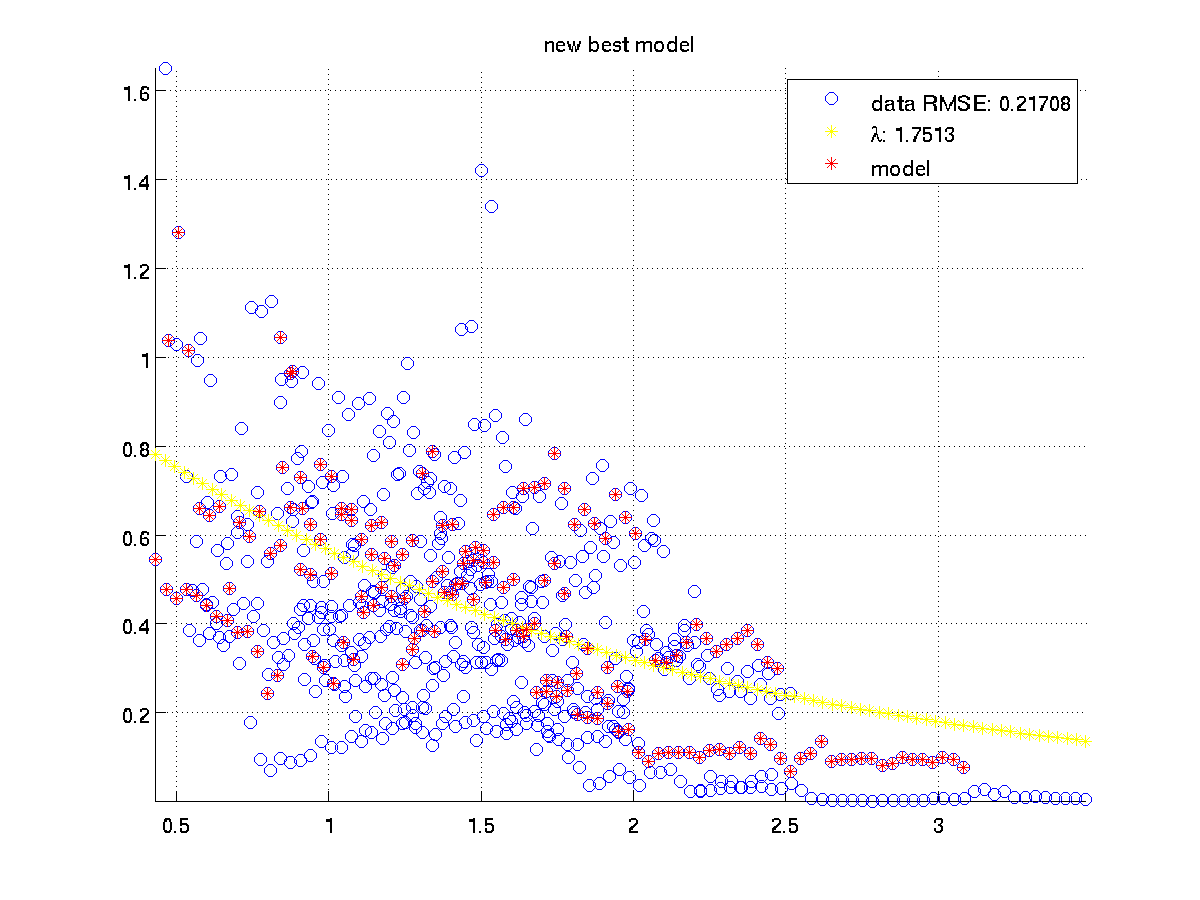
\includegraphics[scale=0.55]{images/ransac1}
	\captionof{figure}{In blu i livelli di contrasto di tutte le features, in rosso quelli del modello e in giallo la curva approssimante candidata.}
	\label{fig:tryLam}
\end{figure}

\noindent Il difetto di questo approccio \`e che vengono presi in considerazione anche dati molto rumorosi, che influiscono in parte sulla bont\`a del risultato.

\begin{figure}[H]
	\centering
	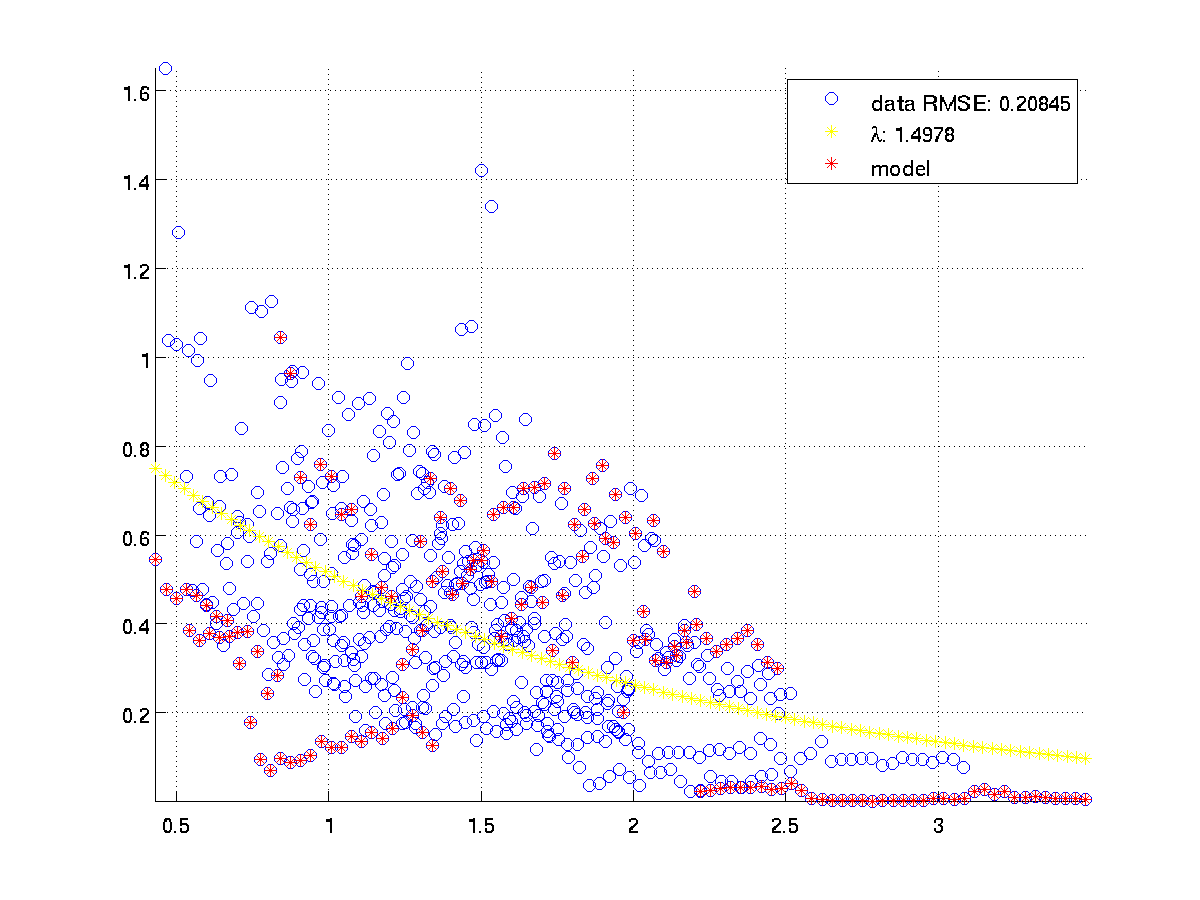
\includegraphics[scale=0.55]{images/ransacWin}
	\captionof{figure}{Miglior curva calcolata da RANSAC. In rosso i valori del modello eletto.}
	\label{fig:ransac}
\end{figure}


\subsection{Stima di $\lambda$ mediante minMax (deprecato)}

\noindent Definita la formula del contrasto per ogni feature come

$$ c_{i,f} = k_fe^{-t_{i,f}/\lambda} $$

\noindent il parametro $k_f$ risulta essere costante all'interno di ogni singola sequenza di corner, mentre $\lambda$ \`e globale.\\
\noindent Sfruttando $k_f$ \`e possibile imporre la seguente uguaglianza fra due campioni di una stessa feature in modo da stimare il parametro $\lambda$ utilizzando i livelli di contrasto massimo e minimo (ed i relativi tempi all'impatto):

$$ c_1e^{t_1/\lambda} = c_2e^{t_2/\lambda} $$
$$ \lambda = \frac{t_2-t_1}{\log\frac{c_1}{c_2}} $$

\noindent A questo punto viene introdotto un primo semplice criterio atto ad eliminare features eccessivamente rumorose: ricordando che i dati sono ordinati sul tempo d'impatto (e quindi il contrasto risulter\`a essere una funzione decrescente) vengono ignorate features la cui differenza fra gli indici dei valori di contrasto minimo e massimo non \`e sufficientemente grande (nel nostro caso deve essere superiore alla met\`a del numero di corners all'interno del set).\\

\noindent Successivamente si pu\`o procedere al calcolo di un $\lambda$ globale in base a quelli stimati calcolandone la media o la mediana.\\

\noindent Tale approccio tuttavia, per quanto computazionalmente leggero, \`e stato abbandonato a causa dell'eccessiva sensibilit\`a all'errore sui dati (dal momento che spesso vengono selezionati come valori di min e max proprio degli outliers). Gli altri due approcci invece facendo uso di una maggiore quantit\`a di dati risultano essere molto pi\`u robusti, ma pagano in termini di prestazioni a causa della complessit\`a dei fitting delle curve.






\chapter{Risultati sperimentali}

\noindent I test sono stati eseguiti sulla sequenza di immagini fornite, consistenti in 113 frames estratti da un video acquisito mediante una telecamera in condizioni di nebbia. Di tale filmato tuttavia non sono noti parametri quali il framerate e la velocit\`a del veicolo; per ovviare a queste incognite sono state fatte diverse assunzioni:
\begin{itemize}
	\item	framerate a 30fps: una diversa frequenza d'acquisizione porterebbe a calcolare diversi tempi d'impatto, ma i valori rimarrebbero comunque congruenti fra di loro. Molto pi\`u rilevante \`e che il framerate si mantenga costante per tutto il filmato.
	\item	moto rettilineo: necessario per semplificare il tracking delle features. Ispezionando il filmato tuttavia si notano delle vistose oscillazioni, possibili cause di problemi in fase di tracking.
	\item	velocit\'a costante: il tempo all'impatto medio (in secondi) si relaziona alla visibilit\`a (in metri) mediante la velocit\`a del veicolo, parametro purtroppo non disponibile. In mancanza di migliori soluzioni questo valore \`e stato ipotizzato come costante, in modo da poter considerare il tempo d'impatto come stima della velocit\`a. Sfortunatamente questa assunzione non appare essere realistica, rendendo incongruenti i tempi calcolati (\`e infatti possibile ottenere uno stesso tti in condizioni di visibilit\`a peggiori semplicemente rallentando).
\end{itemize}
\noindent Come si nota dal campione di immagini mostrate in figura \ref{fig:video} la visibilit\`a migliora nel corso della sequenza.\\

\noindent A causa di risultati poco congruenti registrati nei test mostrati nelle sezioni \ref{fittest} e \ref{ransactest} potenzialmente riconducibili ad una violazione della terza ipotesi \`e stato deciso di acquisire appositamente dei nuovi filmati ad una velocit\`a nota e costante, anche se in condizioni di visibilit\`a ideali (vista la stagione), annotando tutti i parametri necessari per completare i test.\\


\newcommand{\videoScale}{0.5}
\begin{figure}[H]
\centering
\begin{tabular}{ccc}
	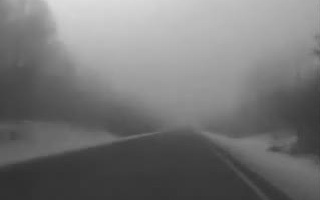
\includegraphics[scale=\videoScale]{images/frame0000.jpg} & 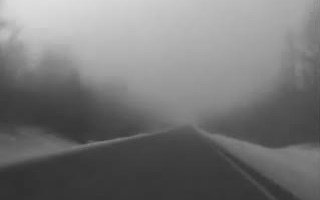
\includegraphics[scale=\videoScale]{images/frame0010.jpg} & 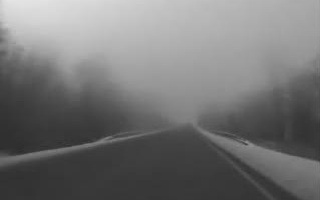
\includegraphics[scale=\videoScale]{images/frame0020.jpg}\\
	frame0000 & frame0010 & frame0020 \\
	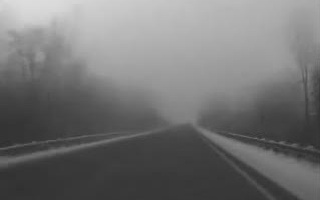
\includegraphics[scale=\videoScale]{images/frame0030.jpg} & 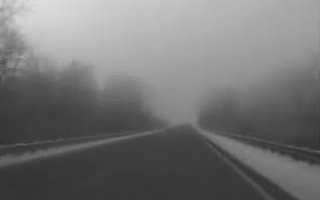
\includegraphics[scale=\videoScale]{images/frame0040.jpg} & 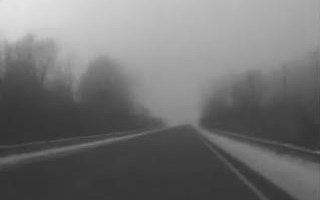
\includegraphics[scale=\videoScale]{images/frame0050.jpg}\\
	frame0030 & frame0040 & frame0050 \\
	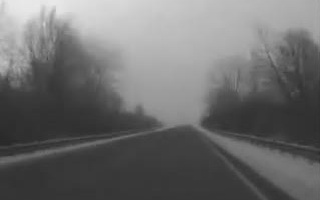
\includegraphics[scale=\videoScale]{images/frame0060.jpg} & 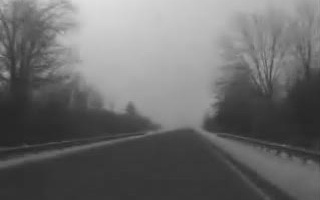
\includegraphics[scale=\videoScale]{images/frame0070.jpg} & 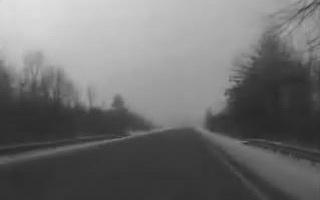
\includegraphics[scale=\videoScale]{images/frame0080.jpg}\\
	frame0060 & frame0070 & frame0080 \\
	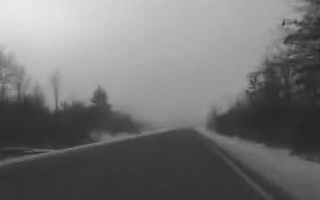
\includegraphics[scale=\videoScale]{images/frame0090.jpg} & 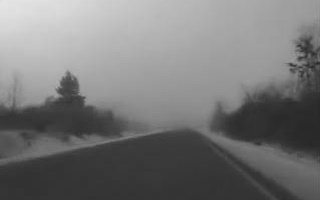
\includegraphics[scale=\videoScale]{images/frame0100.jpg} & 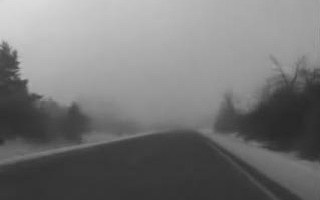
\includegraphics[scale=\videoScale]{images/frame0110.jpg}\\
	frame0090 & frame0100 & frame0110 \\
\end{tabular}
\caption{Campioni estratti dalla sequenza di immagini fornite. Si noti come le condizioni di visibilit\`a migliorano.}
\label{fig:video}
\end{figure}

\section{Calcolo del vanishing pointe e tracking delle features}

\noindent Le figure \ref{fig:vp15}, \ref{fig:vp25} e \ref{fig:vp50} rappresentano il risultato dell'elaborazione dell'algoritmo sul calcolo del vanishing point su differenti sezioni del video con nebbia: l'algoritmo restituisce risultati tanto migliori quanto pi\`u sono le features disponibili, a loro volta dipendenti dal numero di frames; mentre per pochi frames (quindici) il calcolo del vanishing point \`e affetto da errori pi\`u o meno grandi, per tracking pi\`u lunghi (oltre i trenta frames) l'affidabilit\`a dell'algoritmo migliora notevolmente.\\

\noindent Nelle immagini poste a destra \`e possibile verificare come la met\`a delle linee di fuga individuate venga eliminata dal set perch\'e troppo lontana dal vanishing point trovato.\\

\newcommand{\imTrackScale}{0.7}
\begin{figure}[H]
\begin{minipage}[c]{0.5\linewidth}
	\centering
	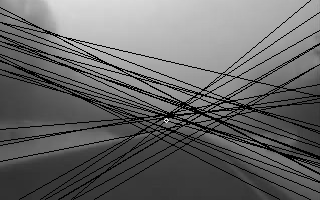
\includegraphics[scale=\imTrackScale]{images/bF_0000_15.png}
	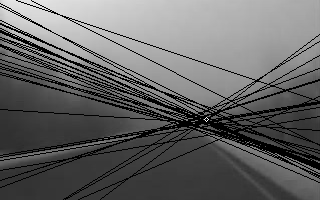
\includegraphics[scale=\imTrackScale]{images/bF_0020_15.png}
	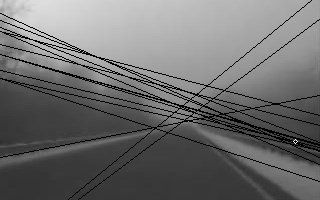
\includegraphics[scale=\imTrackScale]{images/bF_0040_15.png}
	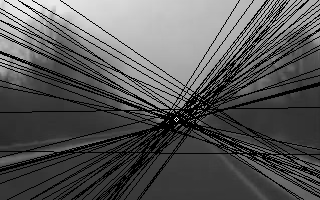
\includegraphics[scale=\imTrackScale]{images/bF_0060_15.png}
\end{minipage}
\begin{minipage}[c]{0.5\linewidth}
	\centering
	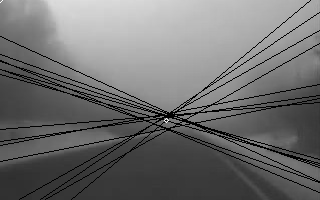
\includegraphics[scale=\imTrackScale]{images/aF_0000_15.png}
	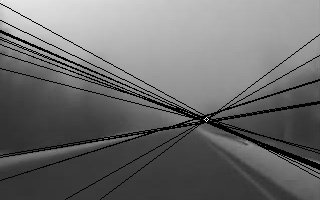
\includegraphics[scale=\imTrackScale]{images/aF_0020_15.png}
	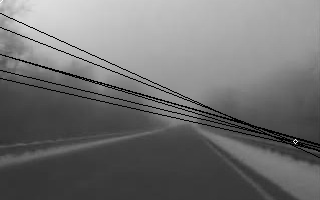
\includegraphics[scale=\imTrackScale]{images/aF_0040_15.png}
	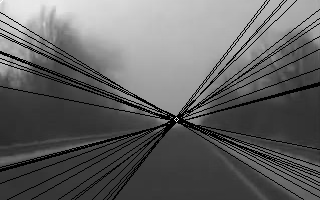
\includegraphics[scale=\imTrackScale]{images/aF_0060_15.png}
\end{minipage}
\caption[short]{A sinistra: linee di fuga per 15 frames a partire dalle immagini 0, 20, 40 e 60. A destra: stesse features dopo il filtro sul vanishing point.}
\label{fig:vp15}
\end{figure}

\begin{figure}[H]
\begin{minipage}[c]{0.5\linewidth}
	\centering
	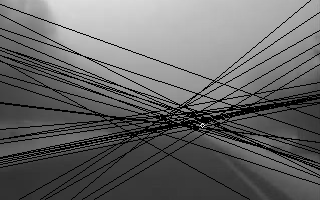
\includegraphics[scale=\imTrackScale]{images/bF_0000_25.png}
	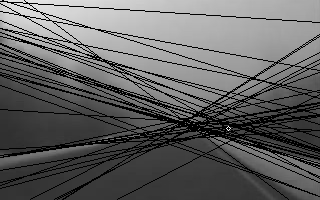
\includegraphics[scale=\imTrackScale]{images/bF_0020_25.png}
	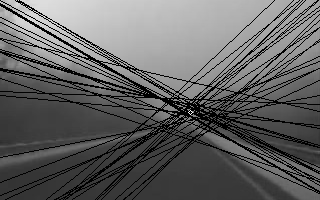
\includegraphics[scale=\imTrackScale]{images/bF_0040_25.png}
	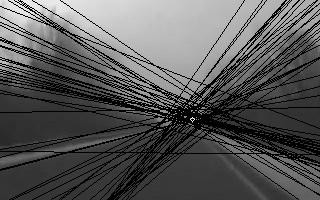
\includegraphics[scale=\imTrackScale]{images/bF_0060_25.png}
\end{minipage}
\begin{minipage}[c]{0.5\linewidth}
	\centering
	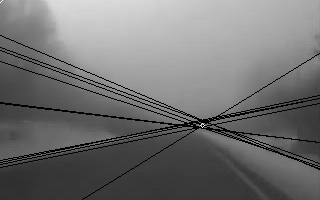
\includegraphics[scale=\imTrackScale]{images/aF_0000_25.png}
	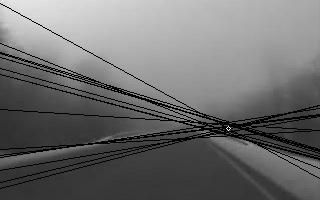
\includegraphics[scale=\imTrackScale]{images/aF_0020_25.png}
	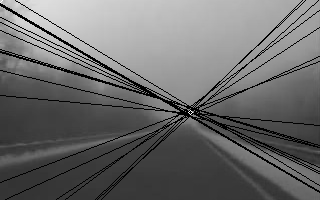
\includegraphics[scale=\imTrackScale]{images/aF_0040_25.png}
	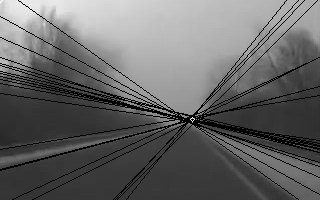
\includegraphics[scale=\imTrackScale]{images/aF_0060_25.png}
\end{minipage}
\caption[short]{A sinistra: linee di fuga per 25 frames a partire dalle immagini 0, 20, 40 e 60. A destra: stesse features dopo il filtro sul vanishing point.}
\label{fig:vp25}
\end{figure}

\begin{figure}[H]
\begin{minipage}[c]{0.5\linewidth}
	\centering
	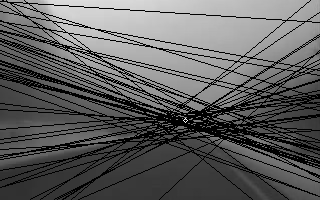
\includegraphics[scale=\imTrackScale]{images/bF_0000_50.png}
	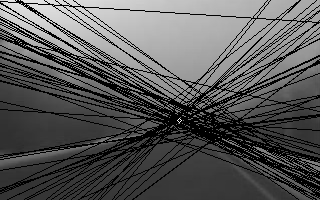
\includegraphics[scale=\imTrackScale]{images/bF_0020_50.png}
	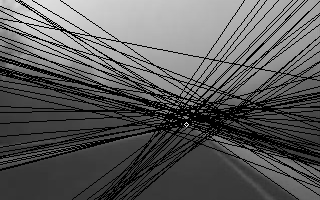
\includegraphics[scale=\imTrackScale]{images/bF_0040_50.png}
	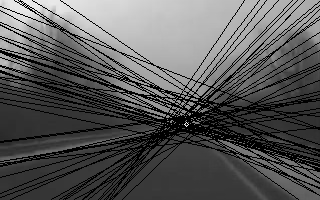
\includegraphics[scale=\imTrackScale]{images/bF_0060_50.png}
\end{minipage}
\begin{minipage}[c]{0.5\linewidth}
	\centering
	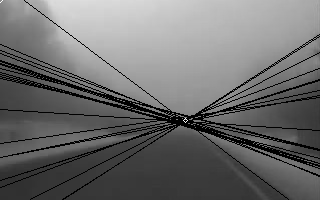
\includegraphics[scale=\imTrackScale]{images/aF_0000_50.png}
	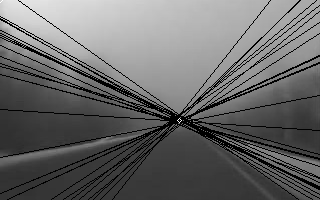
\includegraphics[scale=\imTrackScale]{images/aF_0020_50.png}
	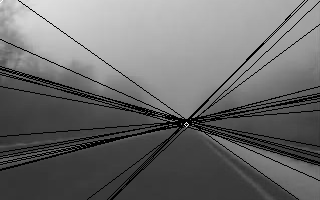
\includegraphics[scale=\imTrackScale]{images/aF_0040_50.png}
	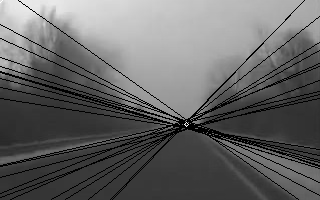
\includegraphics[scale=\imTrackScale]{images/aF_0060_50.png}
\end{minipage}
\caption[short]{A sinistra: linee di fuga per 50 frames a partire dalle immagini 0, 20, 40 e 60. A destra: stesse features dopo il filtro sul vanishing point.}
\label{fig:vp50}
\end{figure}

\noindent L'algoritmo \`e stato testato con diversi punti di partenza e diverse lunghezze di inseguimento, allo scopo di osservare il numero di features restituite. Dal momento che la presenza di RANSAC in fase di calcolo del vanishing point porta ad una certa variabilit\`a del risultato \`e stato considerato il valore medio su dieci esecuzioni per ogni condizione iniziale.\\
\noindent I risultati nella tabella \ref{tabNum} mostrano come il numero di feature estratte aumenti con la lunghezza del tracking e con il migliorare delle condizioni di visibilit\`a. La varianza sul numero di features a parit\`a di condizioni iniziali \`e minima.

\begin{table}[H]
\begin{center}
\begin{tabular}{|c|c|c|c|c|}
	\hline
	& 15 & 25 & 35 & 50 \\
	\hline
	frame0000 & 11 & 12 & 20 & 23\\
	\hline
	frame0020 & 15 & 18 & 18 & 28\\
	\hline
	frame0040 & 6 & 18 & 25 & 25\\
	\hline
	frame0060 & 24 & 23 & 22 & 23\\
	\hline
\end{tabular}
\caption{Numero medio di features estratte dalla sequenza di immagini. Sulle righe l'immagine di partenza, sulle colonne il numero di frame analizzati.}
\label{tabNum}
\end{center}
\end{table}



\newpage
\section{Tempi d'impatto}
\noindent Allo scopo di determinare l'affidabilit\`a dei tempi d'impatto calcolati si \`e deciso di allestire un test per confrontarli con quelli reali utilizzando uno dei nuovi filmati acquisiti: una volta selezionato un insieme di features inseguite correttamente ne viene calcolato il tempo d'impatto rispetto al punto in cui \`e stato acquisito il primo frame (uguale al tti calcolato in una qualsiasi immagine $i$ pi\`u il tempo di frame moltiplicato per $i-1$), valore che verr\`a confrontato con quello effettivo ottenuto dividendo la distanza reale\footnote{In mancanza di strumenti appositi le misurazioni sono state effettuate usando Google Earth.} dell'elemento che ha generato la feature per la velocit\`a del veicolo.\\

\begin{table}[H]
\centering
\begin{tabular}{|c|c|c|c|}
	\hline
	distanza & tti reale & \begin{minipage}{2.5cm}\centering tti calcolato al frame 0 \end{minipage}& errore\\[6pt] \hline
	17m	& 1.53s	& 1.73s	& 0.2s	\\ \hline
	19m	& 1.71s	& 1.9s	& 0.19s	\\ \hline
	20m	& 1.8s	& 2.08s	& 0.28s	\\ \hline
	21m	& 1.89s	& 2.4s	& 0.51s	\\ \hline
	24m	& 2.16s	& 2.22s	& 0.06s	\\ \hline
	32m	& 2.88s	& 2.72s	& 0.16s	\\ \hline
	46m	& 4.14s	& 4.32s	& 0.18s	\\ \hline
	46m	& 4.14s	& 4.76s	& 0.62s	\\ \hline
	46m	& 4.14s	& 5.08s	& 0.94s	\\ \hline
	46m	& 4.14s	& 4.26s	& 0.12s	\\ \hline
	64m	& 5.76s	& 3.86s	& 1.9s	\\ \hline
	64m	& 5.76s	& 5.34s	& 0.42s	\\ \hline

\end{tabular}
\caption{Valori ottenuti viaggiando ad una velocit\`a di 40 km/h.}
\end{table}

\noindent I risultati per i livelli di precisione dei valori considerati (precisione del tachimetro analogico nel misurare la velocit\`a, precisione con cui \`e stata ricostruita la posizione del veicolo nel primo frame, precisione delle distanze misurate) possono considerarsi ampiamente soddisfacenti.\\

\newcommand{\ttiScale}{0.304}
\begin{table}[H]
\centering
\begin{tabular}{|@{}c@{}|@{}c@{}c@{}|@{}c|}
	\hline
	\begin{minipage}[H]{0.35\linewidth}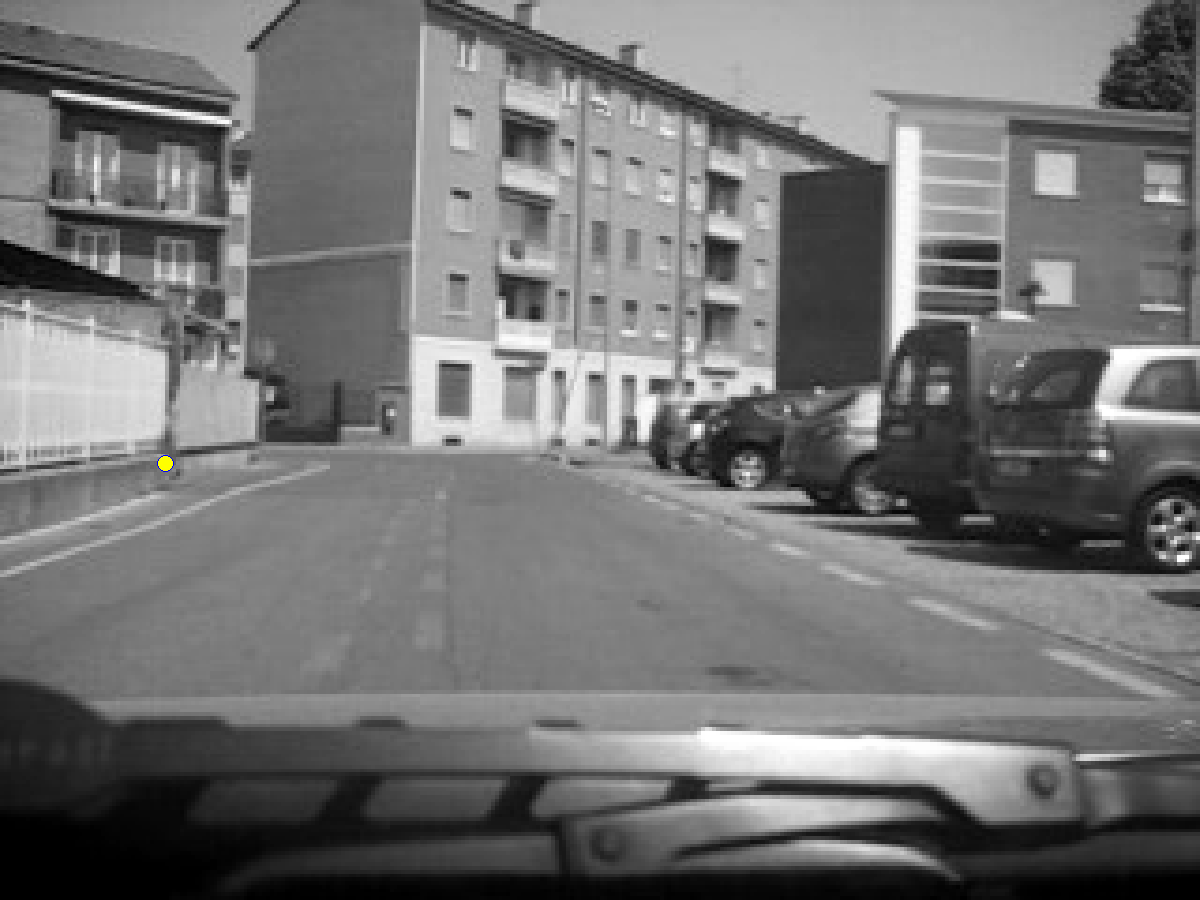
\includegraphics[scale=\ttiScale]{images/tti1.png} \end{minipage} & 
	\begin{minipage}[H]{0.13\linewidth} \begin{tabular}{l} dist: 32m \\ tti_r: 2.88s \\ tti_0: 2.72s \\ err : 0.16s \\ \end{tabular}\end{minipage} & 
	\begin{minipage}[H]{0.35\linewidth}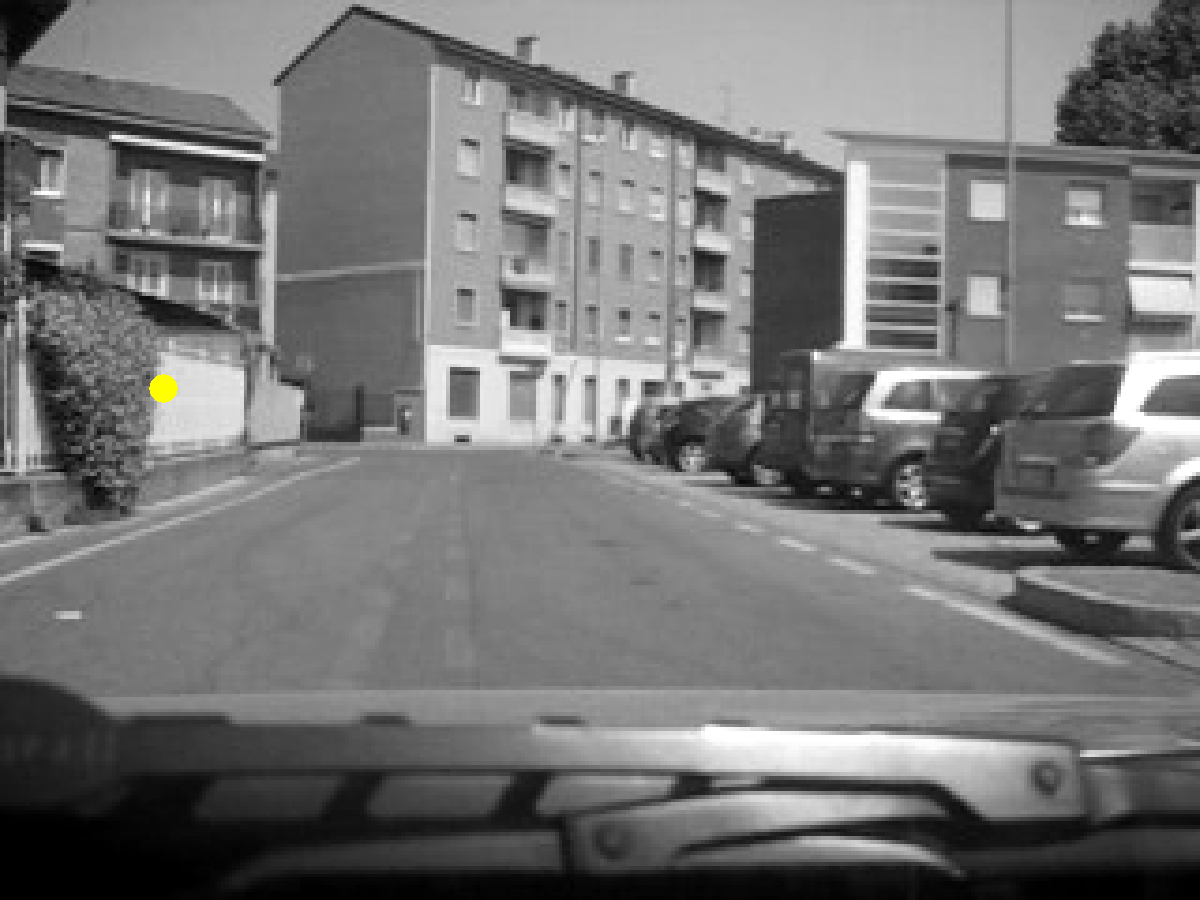
\includegraphics[scale=\ttiScale]{images/tti2.png} \end{minipage} & 
	\begin{minipage}[H]{0.13\linewidth} \begin{tabular}{l} dist: 24m \\ tti_r: 2.16s \\ tti_0: 2.22s \\ err : 0.06s \\ \end{tabular}\end{minipage} \\
	\hline
	\begin{minipage}[H]{0.35\linewidth}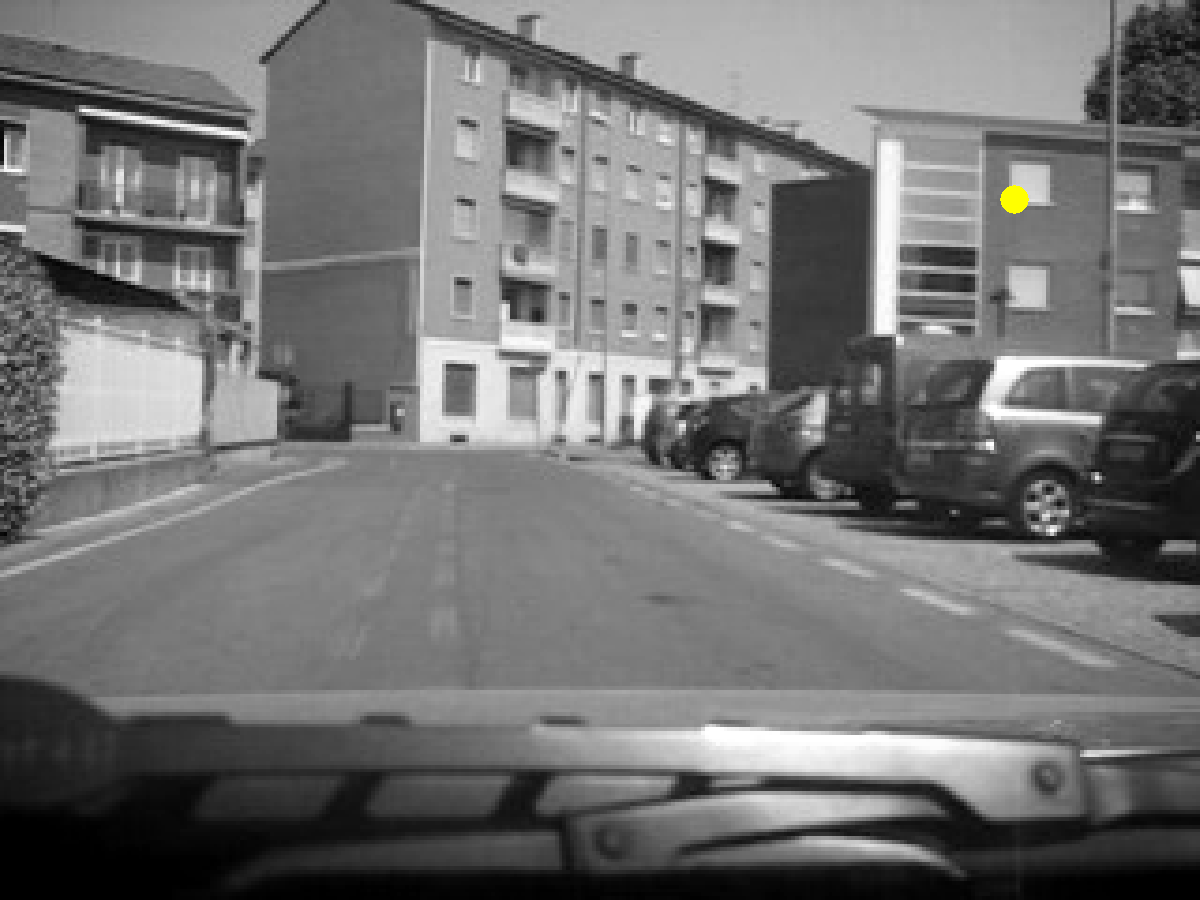
\includegraphics[scale=\ttiScale]{images/tti3.png} \end{minipage} & 
	\begin{minipage}[H]{0.13\linewidth} \begin{tabular}{l} dist: 46m \\ tti_r: 4.14s \\ tti_0: 5.08s \\ err : 0.94s \\ \end{tabular}\end{minipage} & 
	\begin{minipage}[H]{0.35\linewidth}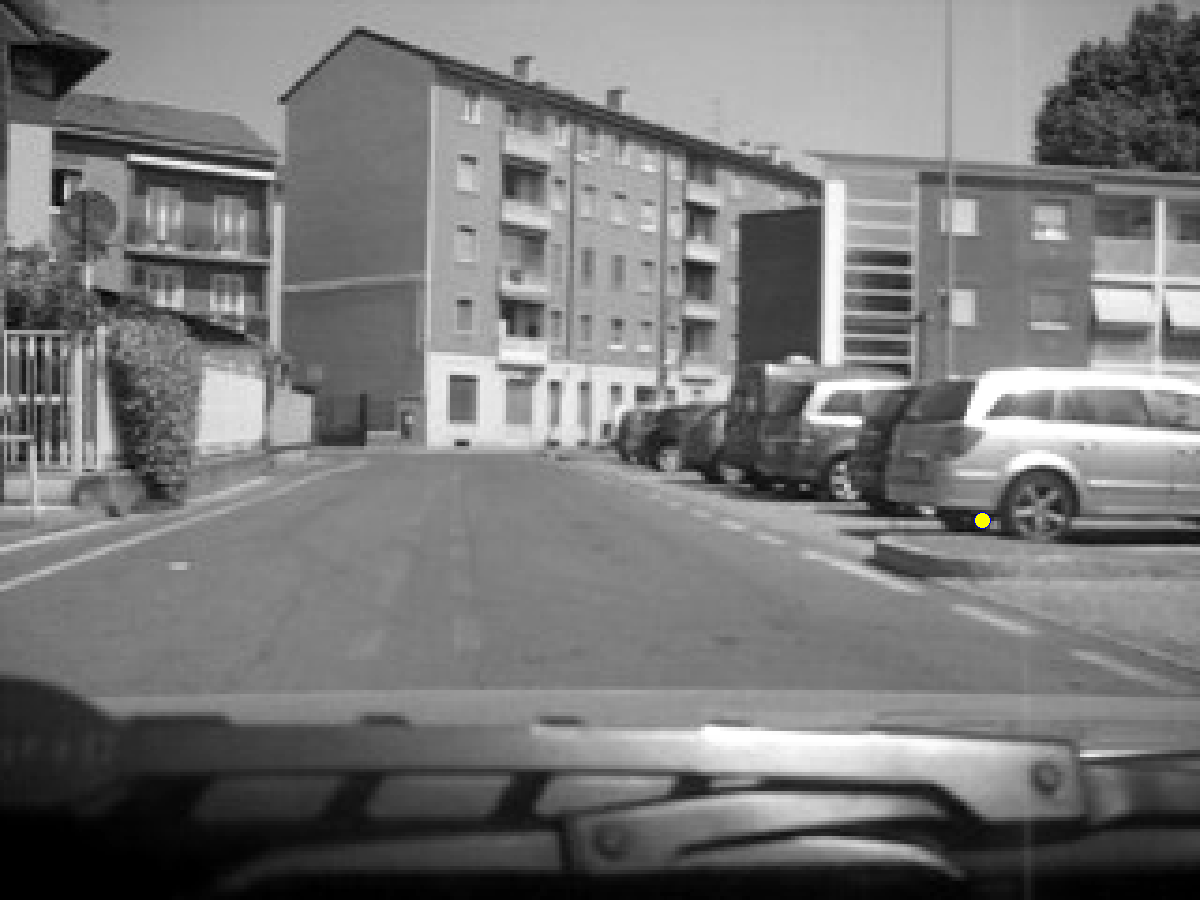
\includegraphics[scale=\ttiScale]{images/tti4.png} \end{minipage} & 
	\begin{minipage}[H]{0.13\linewidth} \begin{tabular}{l} dist: 19m \\ tti_r: 1.71s \\ tti_0: 1.9s \\ err : 0.19s \\ \end{tabular}\end{minipage} \\
	\hline
	\begin{minipage}[H]{0.35\linewidth}\includegraphics[scale=\ttiScale]{images/tti5.png} \end{minipage} & 
	\begin{minipage}[H]{0.13\linewidth} \begin{tabular}{l} dist: 20m \\ tti_r: 1.8s \\ tti_0: 2.08s \\ err : 0.28s \\ \end{tabular}\end{minipage} & 
	\begin{minipage}[H]{0.35\linewidth}\includegraphics[scale=\ttiScale]{images/tti6.png} \end{minipage} & 
	\begin{minipage}[H]{0.13\linewidth} \begin{tabular}{l} dist: 64m \\ tti_r: 5.76s \\ tti_0: 3.86s \\ err : 1.9s \\ \end{tabular}\end{minipage} \\
	\hline
	\begin{minipage}[H]{0.35\linewidth}\includegraphics[scale=\ttiScale]{images/tti7.png} \end{minipage} & 
	\begin{minipage}[H]{0.13\linewidth} \begin{tabular}{l} dist: 46m \\ tti_r: 4.14s \\ tti_0: 4.32s \\ err : 0.18s \\ \end{tabular}\end{minipage} & 
	\begin{minipage}[H]{0.35\linewidth}\includegraphics[scale=\ttiScale]{images/tti8.png} \end{minipage} & 
	\begin{minipage}[H]{0.13\linewidth} \begin{tabular}{l} dist: 64m \\ tti_r: 5.76s \\ tti_0: 5.34s \\ err : 0.42s \\ \end{tabular}\end{minipage} \\
	\hline
\end{tabular}
\caption{Valori ottenuti viaggiando ad una velocit\`a di 40 km/h. In giallo la feature inseguita.}
\end{table}


\newpage
\section{Stima di $\lambda$ mediante fitting}
\label{fittest}

%% FIXME VISUALIZZAZIONE DELLE FEATURES -------------------

\noindent Le figure \ref{fig:feats1}, \ref{fig:feats2}, \ref{fig:feats3} e \ref{fig:feats4} rappresentano i livelli di contrasto (ordinati sul tempo d'impatto) e le relative curve approssimanti di ciascuna delle features trovate analizzando il set di cinquanta fra i frames forniti a partire da \verb|frame0000| del video con nebbia. Appare palese come i dati siano rumorosi, spesso portando a stimare parametri inverosimili.\\

\newcommand{\imFeat}{.42}
\begin{figure}[H]
\begin{minipage}[t]{0.5\linewidth}
	\centering
	feat1 - $k: 10.81, \lambda: 1.5 $\\
	\includegraphics[scale=\imFeat]{images/feat1}\\
	feat3 - $k: 8.05, \lambda: 2.62 $\\
	\includegraphics[scale=\imFeat]{images/feat3}\\
\end{minipage}
\begin{minipage}[t]{0.5\linewidth}
	\centering
	feat2 - $k: 10.3, \lambda: 1.69 $\\
	\includegraphics[scale=\imFeat]{images/feat2}\\
	feat4 - $k: 24.99, \lambda: 1.1 $\\
	\includegraphics[scale=\imFeat]{images/feat4}\\
\end{minipage}
\caption[short]{Features e relative curve fittate. I dati sono ordinati in base al tempo d'impatto.}
\label{fig:feats1}
\end{figure}

\begin{figure}[H]
\begin{minipage}[t]{0.5\linewidth}
	\centering
	feat5 - $k: 17.16, \lambda: 400.55 $\\
	\includegraphics[scale=\imFeat]{images/feat5}\\
	feat7 - $k: 18.09, \lambda: 1.22 $\\
	\includegraphics[scale=\imFeat]{images/feat7}\\
	feat9 - $k: 6.35, \lambda: 2.28 $\\
	\includegraphics[scale=\imFeat]{images/feat9}\\
\end{minipage}
\begin{minipage}[t]{0.5\linewidth}
	\centering
	feat6 - $k: 3.76, \lambda: 43672 $\\
	\includegraphics[scale=\imFeat]{images/feat6}\\
	feat8 - $k: 6.17, \lambda: 2.24 $\\
	\includegraphics[scale=\imFeat]{images/feat8}\\
	feat10 - $k: 402.16, \lambda: 0.61 $\\
	\includegraphics[scale=\imFeat]{images/feat10}\\
\end{minipage}
\caption[short]{Features e relative curve fittate. I dati sono ordinati in base al tempo d'impatto.}
\label{fig:feats2}
\end{figure}

\begin{figure}[H]
\begin{minipage}[t]{0.5\linewidth}
	\centering
	feat11 - $k: 12.4, \lambda: 0.91 $\\
	\includegraphics[scale=\imFeat]{images/feat11}\\


	feat13 - $k: 16.76, \lambda: 3.04 $\\
	\includegraphics[scale=\imFeat]{images/feat13}\\
	feat15 - $k: 21.28, \lambda: 1.09 $\\
	\includegraphics[scale=\imFeat]{images/feat15}\\
\end{minipage}
\begin{minipage}[t]{0.5\linewidth}
	\centering
	feat12 - $k: 11.65, \lambda: 1.4 $\\
	\includegraphics[scale=\imFeat]{images/feat12}\\
	feat14 - $k: 10.11, \lambda: 12.4 $\\
	\includegraphics[scale=\imFeat]{images/feat14}\\
	feat16 - $k: 6.09, \lambda: 2.82 $\\
	\includegraphics[scale=\imFeat]{images/feat16}\\
\end{minipage}
\caption[short]{Features e relative curve fittate. I dati sono ordinati in base al tempo d'impatto.}
\label{fig:feats3}
\end{figure}

\begin{figure}[H]
\begin{minipage}[t]{0.5\linewidth}
	\centering
	feat17 - $k: 2.09, \lambda: 23824.37 $\\
	\includegraphics[scale=\imFeat]{images/feat17}\\
	feat19 - $k: 22.84, \lambda: 0.52 $\\
	\includegraphics[scale=\imFeat]{images/feat19}\\
	feat21 - $k: 179.3, \lambda: 0.13 $\\
	\includegraphics[scale=\imFeat]{images/feat21}\\
\end{minipage}
\begin{minipage}[t]{0.5\linewidth}
	\centering
	feat18 - $k: 2.04, \lambda: 2.63 $\\
	\includegraphics[scale=\imFeat]{images/feat18}\\
	feat20 - $k: 46.83, \lambda: 0.8 $\\
	\includegraphics[scale=\imFeat]{images/feat20}\\
	feat22 - $k: 38.25, \lambda: 0.73 $\\
	\includegraphics[scale=\imFeat]{images/feat22}\\
\end{minipage}
\caption[short]{Features e relative curve fittate. I dati sono ordinati in base al tempo d'impatto.}
\label{fig:feats4}
\end{figure}



%% DATI MIGLIORI E PEGGIORI ----------------------------------
\newapage
\noindent L'immagine \ref{fig:bestIntErr} invece illustra il quartile dei migliori dati calcolato usando l'area fra i due successivi fitting (ricordiamo che partiamo dall'idea che per buoni set le due curve non differiscono molto). In blu viene visualizzata la curva approssimante l'intero set di dati, mentre in rosso \`e evidenziata la met\`a dei dati con errore minore e la curva approssimante da questi ultimi ottenuta. Similmente, in figura \ref{fig:worstIntErr} sono riportate le features con errore peggiore.\\

\noindent In base ai parametri $\lambda$ delle features migliori viene infine calcolata la mediana come valore globale, mostrato in figura \ref{fig:intErrHist}

\newcommand{\imFeatBW}{.48}
\begin{figure}[H]
\begin{minipage}[t]{0.5\linewidth}
	\centering
	\includegraphics[scale=\imFeatBW]{images/best1}\\
	\includegraphics[scale=\imFeatBW]{images/best3}\\
	\includegraphics[scale=\imFeatBW]{images/best5}\\
\end{minipage}
\begin{minipage}[t]{0.5\linewidth}
	\centering
	\includegraphics[scale=\imFeatBW]{images/best2}\\
	\includegraphics[scale=\imFeatBW]{images/best4}\\
	\includegraphics[scale=\imFeatBW]{images/best6}\\
\end{minipage}
\caption[short]{Migliori features secondo l'integrale dell'errore.}
\label{fig:bestIntErr}
\end{figure}

\begin{figure}[H]
\begin{minipage}[t]{0.5\linewidth}
	\centering
	\includegraphics[scale=\imFeatBW]{images/worst1}\\
	\includegraphics[scale=\imFeatBW]{images/worst3}\\
	\includegraphics[scale=\imFeatBW]{images/worst5}\\
\end{minipage}
\begin{minipage}[t]{0.5\linewidth}
	\centering
	\includegraphics[scale=\imFeatBW]{images/worst2}\\
	\includegraphics[scale=\imFeatBW]{images/worst4}\\
	\includegraphics[scale=\imFeatBW]{images/worst6}\\
\end{minipage}
\caption[short]{Feature peggiori secondo l'integrale dell'errore.}
\label{fig:worstIntErr}
\end{figure}

%% ISTOGRAMMI -----------------------------------

\begin{figure}[H]
	\centering
	\includegraphics[scale=.5]{images/intErrhistLamFit}
	\caption{Istogramma dei migliori $\lambda$ secondo l'integrale dell'errore (mediana: 1.22).}
	\label{fig:intErrHist}
\end{figure}

\noindent Sono infine stati analizzati i diversi valori di $\lambda$ restituiti dal presente algoritmo al variare del numero di frame analizzati e dal frame di partenza; ogni test \`e stato eseguito dieci volte per verificare anche la ripetibilit\`a dei risultati a causa della componente stocastica introdotta da RANSAC nella determinazione del punto di fuga.\\

\begin{table}[H]
\begin{center}
\begin{tabular}{|c|c|c|c|c|}
	\hline
	& 15 & 25 & 35 & 50 \\
	\hline
	frame0000 & 0.51242 (2.2294e-07) & 1.0259 (0.13114) & 0.92892 (0.27711) & 1.217 (0.27272)\\ \hline
	frame0020 & 0.94626 (0.023624) & 0.83583 (0.35476) & 0.75068 (0.16246) & 1.0123 (0.12878)\\ \hline
	frame0040 & 0.52983 (0.073719) & 0.59726 (0.032103) & 0.68024 (0.05821) & 0.92369 (0.067124)\\ \hline
	frame0060 & 0.6039 (0.061717) & 0.60004 (0.084892) & 0.7747 (0.0087826) & 0.72864 (0.059721)\\ \hline
\end{tabular}
\caption{Media (deviazione standard campionaria) del $\lambda$ calcolato mediante fitting. Sulle righe l'immagine di partenza, sulle colonne il numero di frame analizzati.}
\label{tabFit}
\end{center}
\end{table}

\noindent Osservando il filmato campione ci si aspetterebbe di osservare un miglioramento nelle condizioni di visibili\`a, cosa non evidente dai valori restituiti. Tali incongruenze potrebbero essere imputabili a possibili variazioni della velocit\`a nel veicolo usato per l'acquisizione del filmato, in violazione delle ipotesi fatte in partenza. Per questo motivo l'esperimento \`e stato ripetuto utilizzando i nuovi filmati acquisiti: diverse sequenze di immagini sono state estratte da un filmato ripreso con una videocamera a 30fps su di un veicolo alla velocit\`a costante di 60 km/h (precisione ottenibile con un tachimetro analogico) in condizioni di visibilit\`a ideali. Ciascuna sequenza \`e stata analizzata dieci volte.\\

\begin{table}[H]
\centering
\begin{tabular}{|c|c|c|c|c|}
	\hline
	& 15 & 25 & 35 & 50 \\ \hline
	Images01/frame0000.png & 1.57s (0.18s) & 2.01s (0.63s) & 1.27s (0.18s) & 1.57s (0.45s) \\ \hline
	Images02/frame0000.png & 1.20s (0.08s) & 0.95s (0.18s) & 1.12s (0.14s) & 1.34s (0.08s) \\ \hline
	Images02/frame0060.png & 1.4s (0.28s) & 1.22s (0.12s) & 1.15s (0.09s) & 1.39s (0.14s)\\ \hline
	Images03/frame0000.png & 1.02s (0.94s) & 1.17s (0.06s) & 1.34s (0.19s) & 1.37s (0.03s) \\ \hline
	Images04/frame0000.png & 1.57s (0.18s) & 2.01s (0.63s) & 1.27s (0.18s) & 1.57s (0.45s) \\ \hline
	Images04/frame0040.png & 1.2s (0.08s) & 0.95s (0.18s) & 1.12s (0.14s) & 1.34s (0.08s) \\ \hline
	Images05/frame0000.png & 1.24s (0.02s) & 1.65s (0.01s) & 1.87s (0.35s) & 1.5s (0.05s) \\ \hline
	Images05/frame0100.png & 1.4s (0.28s) & 1.22s (0.12s) & 1.15s (0.09s) & 1.39s (0.14s) \\ \hline
\end{tabular}
\caption{$\lambda$ medio e deviazione standard campionaria per diversi frame iniziali e lunghezze d'analisi.}
\end{table}

\noindent Si nota come all'aumentare della lunghezza dell'analisi le soluzioni tendano a convergere, essendo le condizioni di visibilit\`a sostanzialmente identiche nelle diverse sequenze. Per un $\lambda$ pari ad 1.4s ad una velocit\`a di 60 km/h la visibilit\`a risulta essere di 23.3m\\

\noindent Ricordiamo che il $\lambda$ ottenuto corrisponde alla distanza media per cui la curva teorica del contrasto delle varie features raggiunge il valore $k_f/e$, scelto in quanto comodo per i calcoli, e non va quindi interpretato come visibilit\`a in termini ``umani'': per far ci\`o si dovrebbe determinare un valore percentuale $q$ sul contrasto raggiunto il quale una feature campione pu\`o essere considerata visibile per un occhio umano, per poi riscalare i valori ottenuti mediante un coefficiente $\alpha$ (pari a $-log\left(q\right)$) come nella formula

$$qk_f = k_fe^{-t_{imp,q}/\lambda}$$
$$t_{imp,q} = -\lambda\log \left(q\right) = \alpha\lambda$$

\noindent ricordando che $q$ \`e inferiore all'unit\`a e quindi $\alpha$ risulter\`a essere positivo. \\
\noindent Quindi una volta calcolato il $\lambda$ come mostrato fin'ora potremo moltiplicarlo per $\alpha$ ottenendo la distanza cui la feature assume il livello $qk_f$ per cui possiamo considerarla come visibile.\\


\newpage
\section{Stima di $\lambda$ mediante RANSAC}
\label{ransactest}

\noindent Lo stesso set di features della sezione precedente viene utilizzato per stimare il $\lambda$ globale mediante RANSAC, di cui sono riportate alcune iterazioni nelle seguenti immagini.

\newcommand{\imFeatRan}{0.45}
\begin{figure}[H]
\begin{minipage}[t]{0.5\linewidth}
	\centering
	\includegraphics[scale=\imFeatRan]{images/ransac1}\\
	\includegraphics[scale=\imFeatRan]{images/ransac3}\\
%	\includegraphics[scale=\imFeatRan]{images/ransac5}\\
\end{minipage}
\begin{minipage}[t]{0.5\linewidth}
	\centering
	\includegraphics[scale=\imFeatRan]{images/ransac2}\\
	\includegraphics[scale=\imFeatRan]{images/ransac4}\\
%	\includegraphics[scale=\imFeatRan]{images/ransac6}\\
\end{minipage}
\caption[short]{Esempio di iterazioni di RANSAC. In blu i dati, in giallo le curva candidata, in rosso i campioni del relativo modello.}
\label{fig:ransac1}
\end{figure}

\begin{figure}[H]
\begin{minipage}[t]{0.5\linewidth}
	\centering
	\includegraphics[scale=\imFeatRan]{images/ransac7}\\
	\includegraphics[scale=\imFeatRan]{images/ransac9}\\
	\includegraphics[scale=\imFeatRan]{images/ransac11}\\
\end{minipage}
\begin{minipage}[t]{0.5\linewidth}
	\centering
	\includegraphics[scale=\imFeatRan]{images/ransac8}\\
	\includegraphics[scale=\imFeatRan]{images/ransac10}\\
	\includegraphics[scale=\imFeatRan]{images/ransac12}\\
\end{minipage}
\caption[short]{Esempio di iterazioni di RANSAC. In blu i dati, in giallo le curva candidata, in rosso i campioni del relativo modello.}
\label{fig:ransac2}
\end{figure}

\begin{figure}[H]
	\centering
	\includegraphics[scale=.7]{images/ransacWin}
	\caption{Migliore curva trovata mediante RANSAC. $\lambda: 1.5$.}
	\label{fig:ransacWin}
\end{figure}

\noindent Allo scopo di verificare la variabilit\`a dei risultati di RANSAC \`e stato ripetuto il calcolo per cinquanta volte sullo stesso set di features.

\begin{figure}[H]
	\centering
	\includegraphics[scale=.6]{images/multiRansac}
	\caption{Istogramma dei $\lambda$ ottenuti eseguendo RANSAC cinquanta volte sullo stesso set di dati.}
	\label{fig:multiRansac}
\end{figure}

\noindent In modo analogo al caso precedente, l'algoritmo \`e stato eseguito dieci volte sul video con nebbia per diverse condizioni iniziali, con risultati ancora una volta difficilmente interpretabili.

\begin{table}[H]
\begin{center}
\begin{tabular}{|c|c|c|c|c|}
	\hline
	& 15 & 25 & 35 & 50 \\ \hline
	Images/frame0000.jpg & 0.77s (0.01s) & 0.71s (0.005s) & NaN (NaN) & 1.42s (0.02s)\\ \hline
	Images/frame0020.jpg & 0.59s (0.01s) & 0.96s (0.12s) & 1.06s (0.06s) & 0.83s (0.003s)\\ \hline
	Images/frame0040.jpg & 0.84s (1.2e-16s) & 0.51s (0.002s) & 0.58s (0.003s) & 0.99s (0.007s)\\ \hline
	Images/frame0060.jpg & 0.38s (0.001s) & 0.6s (0.08s) & 0.55s (0.06s) & 1.06s (0.06s)\\ \hline
\end{tabular}
\caption{Media (deviazione standard campionaria) del $\lambda$ calcolato mediante RANSAC. Sulle righe l'immagine di partenza, sulle colonne il numero di frame analizzati. I NaN indicano il fallimento di RANSAC a causa dell'eccessiva rumorosit\`a dei dati (l'eccessivo errore medio non ha portato a nessun set di consenso abbastanza grande).}
\label{tabRans}
\end{center}
\end{table}

\noindent Il test \`e stato quindi ripetuto utilizzando le nuove sequenze di immagini acquisite:

\begin{table}[H]
\begin{center}
\begin{tabular}{|c|c|c|c|c|}
	\hline
	& 15 & 25 & 35 & 50 \\ \hline
	Images01/frame0000.png & 1.43s (0.08s) & 2.03s (0.16s) & 0.9s (0.02s) & 1.14s (0.14s)\\ \hline
	Images02/frame0000.png & 1.22s (0.03s) & 1.99s (0.11s) & 1.58s (0.16s) & 1.8s (0.11s)\\ \hline
	Images02/frame0060.png & 2.8s (0.25s) & 1.55s (1.1s) & 3.68s (0.71s) & 2.95s (0.18s)\\ \hline
	Images03/frame0000.png & 0.17s (0.00s) & 0.56s (0.08s) & 0.67s (0.11s) & 1.01s (0.09s)\\ \hline
	Images04/frame0000.png & 45.3s (8.7s) & 1.87s (0.14s) & 1.13s (0.21s) & 1.63s (0.11s)\\ \hline
	Images04/frame0040.png & 0.54s (0.22s) & 2.73s (0.26s) & 2.33s (0.28s) & 2.26s (0.19s)\\ \hline
	Images05/frame0000.png & 0.87s (0.04s) & 1.02s (0.042s) & 3.97s (1.3s) & 1.65s (0.36s)\\ \hline
	Images05/frame0100.png & 0.90s (0.03s) & 0.89s (0.02s) & 0.95s (0.04s) & 0.68s (0.1s)\\ \hline
\end{tabular}
\caption{Media (deviazione standard campionaria) del $\lambda$ calcolato mediante RANSAC sulle nuove sequenze acquisite. Sulle righe l'immagine di partenza, sulle colonne il numero di frame analizzati.}
\label{tab:ransNew}
\end{center}
\end{table}

\noindent I risultati, per quanto molto pi\`u variabili, sembrano avvicinarsi a quelli ottenuti nell'analogo test usanto il metodo di fitting. Un simile risultato era prevedibile dal momento che vengono usati meno filtri sulla bont\`a delle features.



\chapter{Conclusioni e sviluppi futuri}

\noindent I risultati dei test hanno evidenziato come il problema sia fortemente influenzato dal numero di outliers derivati sia da un errato tracking delle features, sia da una non perfetta variazione del contrasto sulle features stesse. Il maggior sforzo computazionale \`e infatti da attribuire alla complessit\`a degli algoritmi utilizzati per escludere gli outliers in tutte le fasi dell'elaborazione in modo da avere valori attendibili in ogni condizione.\\

\noindent Sono stati analizzati diversi approcci ed algoritmi per la risoluzione del problema, e si \`e preferito, in ultimo, sacrificare il tempo di elaborazione in favore di una migliore affidabilit\`a dei risultati: gli algoritmi utilizzati sono in grado di individuare autonomamente le features migliori e scartare quelle meno buone, ottenendo dei buoni risultati come esposto nei capitoli precedenti.\\

\noindent Per quanto alcuni degli esperimenti usando il campione video fornito fossero inconcludenti a causa della mancanza di informazioni, i valori ottenuti nei test in condizioni di visibilit\`a ideale hanno comunque mostrato un certo grado di consistenza degli algoritmi implementati. Rimane tuttavia necessario testarli in condizioni di nebbia avendo a disposizione tutte le necessarie informazioni per una corretta valutazione.\\

\noindent \`E inoltre necessario uno studio su come manipolare il $\lambda$ restituito in modo da conferirgli un significato pi\`u vicino al mondo delle percezioni umane, pi\'u intuitivo per l'utente, in modo simile a come suggerito alla fine della sezione \ref{fittest}.\\

\noindent L'aggiunta di un sistema stereoscopico potrebbe migliorare la fase di tracking delle feature, permettendo eliminare quelle inseguite in modo scorretto confrontandone la velocit\`a calcolata con quella effettiva del veicolo.\\

\noindent Ulteriori sviluppi futuri possono riguardare la reimplementazione in C\verb|++| del codice Matlab ed un'ottimizzazione degli algoritmi mirata a migliorarne le performance, eventualmente fino al punto di rendere possibile l'analisi direttamente su uno streaming video in realtime, senza le rielaborazioni successive del codice attualmente in uso.\\




\chapter{Documentazione}


Viene qui presentata una panoramica delle funzioni realizzate. Per informazioni pi\`u dettagliate circa il loro utilizzo consultare l'\verb|help| delle funzioni.

\section[C++]{C\verb_++_}

\paragraph*{\verb_findFeatures:_} \`e la funzione principale dell'algoritmo, si occupa di chiamare le sottoprocedure dell'algoritmo

\paragraph*{\verb_iaasFindCorners:_} estrae dall'immagine i corner con autovalori pi\`u alti

\paragraph*{\verb_iaasTrackCorners:_} cerca di rintracciare i corner della prima immagine (gi\`a calcolati) nella seconda utilizzando l'algoritmo di \emph{Lucas-Kanade}

\paragraph*{\verb_verifyNewFeatureIsOk:_} verifica che un nuovo corner estratto sia coerente con quelli in precedenza rilevati

\paragraph*{\verb_getAroundContrast:_} calcola il contrasto nell'intorno di una feature usando RMS: $$ c\left(I_{M\times N}\right) = \sqrt{\frac{1}{MN}\sum_{i=1}^N\sum_{j=1}^M(i_{ij}-\bar{I})^2} $$

\paragraph*{\verb_verifyValidFeature:_} verifica che una sequenza di corner estratti sia coerente con il movimento e la cross ratio attesa

\paragraph*{\verb_printFeatures:_} scrive sul file la lista di features valide come:
\begin{verbatim}
	     primoFrame numeroFrame [xCoord yCoord contrasto tti]+
\end{verbatim}


\section{Matlab}

\paragraph*{\verb_iaas:_} funzione principale, parsa le feature generate dal codice C\verb|++| e chiede all'utente di selezionare l'algoritmo per il calcolo del $\lambda$ globale.

\paragraph*{\verb_parseFeatures:_} effettua il parsing del file di output generato da \verb|printFeatures| e restituisce una lista di struct contenente le informazioni di ogni feature: \verb|start| \`e il numero della prima immagine in cui appare la feature, \verb|num| il numero di frame nei quali viene inseguita, \verb|x|, \verb|y|, \verb|contr| e \verb|tti| sono array rappresentanti le coordinate, il contrasto e il tempo all'impatto della feature all'interno nell'i-esimo frame in cui vengono individuate. Nelle seguenti funzioni, quando si far\`a riferimento a liste di features si intender\`a cos\`i strutturate.

\paragraph*{\verb_fitLamContr:_} calcola i parametri della curva best fit sui dati di ciascuna delle features fornite in ingresso, aggiungendo il campo \verb|bestData| degli indici del $50\%$ dei corner con valori di contrasto con errore minimo rispetto alla stima. Viene poi aggiunto l'attributo \verb|pars| contenente i parametri del refitting usando il set \verb|bestData|. Vengono inoltre aggiunti diversi attributi per stimare la bont\`a del set di dati che compongono la singola feature (per una lista esaustiva si rimanda all'help della funzione), fra i quali in particolare ricordiamo \verb|intErr|, che calcola l'area fra le curve dei due successivi fit.

\paragraph*{\verb_estimateLamFit:_} seleziona il quartile delle migliori features usando uno degli attributi calcolati da \verb|fitLamContr| (nel nostro caso abbiamo preferito usare l'errore integrale) e usa la mediana dei $\lambda_f$ stimati per calcolare il parametro globale.

\paragraph*{\verb_fitNormContr:_} calcola il $\lambda$ globale mediante RANSAC dopo aver riscalato i livelli di contrasto di ogni feature in base al valore $k_f$ della curva best fit.

\paragraph*{\verb_normContrast:_} normalizza il contrasto di ogni set di features utilizzando diverse possibili tecniche (per una lista completa si rimanda all'help della funzione). Riportiamo l'opzione \verb|fit|, dal momento che \`e quella pi\`u efficace (e di fatto utilizzata all'interno del progetto), che riscala i contrasti delle singole features in base al $k_f$ della curva che meglio approssima il set di dati.

\paragraph*{\verb_myRansac:_} implementazione di RANSAC per calcolare il parametro $\lambda$ della funzione del contrasto dati in ingresso una lista di features.

\paragraph*{\verb_inspectFeatures:_} stampa a video le sequenze di features per un'ispezione visiva, visualizzandone i relativi valori di contrasto.


\paragraph*{\verb_inspectContrasts:_} data una serie di features ne stampa a video i livelli di contrasto ordinati sul tempo d'impatto.

\paragraph*{\verb_michelsonContrast:_} date le coordinate di una feature e la relative immagine restituisce il livello di contrasto nell'intorno come $$c\left(I\right) = \frac{\max(I)-\min(I)}{\max(I)+\min(I)}$$

\paragraph*{\verb_rsmContrast:_} date le coordinate di una feature e la relativa immagine calcola il livello di contrasto nell'intorno come $$ c\left(I_{M\times N}\right) = \sqrt{\frac{1}{MN}\sum_{i=1}^N\sum_{j=1}^M(i_{ij}-\bar{I})^2} $$

\paragraph*{\verb_weberContrast:_} date le coordinate di una feature e la relative immagine calcola il livello di contrasto come $$c\left(i_{i,j}\right)= \frac{i_{i,j}-I_b}{I_b}$$ dove $I_b$ \`e il livello della nebbia.



\chapter{Installazione}
\noindent Il programma \`e stato sviluppato per mezzo di C\verb|++| e Matlab. Per la parte in C\verb|++| \`e necessario essere provvisti delle librerie di OpenCV.\\
L'ultima versione del codice \`e liberamente scaricabile mediante SVN dalla repository messa a disposizione su Google Code all'indirizzo \url{http://code.google.com/p/iaasfog}.
\section{OpenCV}

OpenCV (Open Source Computer Vision) \`e una libreria di funzioni per la computer vision, inizialmente sviluppata da Intel e ora distribuita sotto licenza open source. \`E possibile scaricare l'ultima versione all'indirizzo \url{http://sourceforge.net/projects/opencvlibrary/} \footnote{guida d'installazione ufficiale all'indirizzo \url{http://opencv.willowgarage.com/wiki/InstallGuide}}.

\subsection{Windows}

Per compilare la libreria \`e necessario installare gli header offerti da MinGW (\url{http://http://www.mingw.org/}) e CMake (\url{http://www.cmake.org/cmake/resources/software.html}).\\
\noindent Una volta assicuratisi che il path dei binari di MinGW \`e fra le variabili di ambiente configurare OpenCV mediante l'interfaccia di CMake.

\subsection{Linux / MacOSX}

\noindent Per l'installazione \`e necessario disporre di \verb|cmake|, inoltre devono essere soddisfatte le seguenti dipendenze:
\begin{itemize}
\item \verb|ffmpeg|
\item \verb|libxine-ffmpeg|
\item \verb|libavcodec-dev|
\item \verb|pgk-config|
\item \verb|libgtk2.0-dev|
\end{itemize}

\noindent reperibili mediante \verb|apt-get| o package manager.\\

\noindent Una volta scaricata e scompattata l'ultima versione di OpenCV (2.2.0 alla stesura del presente documento), creare una cartella dove verranno salvate le librerie configurate mediante \verb|cmake| e aprirla con una finestra di terminale. Nel nostro esempio la creeremo nella stessa cartella scompattata

\begin{verbatim}
	$ cd OpenCV2.2.0/
	$ mkdir release; cd release
\end{verbatim}

\noindent Lanciare quindi il comando

\begin{verbatim}
	$ cmake -D CMAKE_BUILD_TYPE=RELEASE -D CMAKE_INSTALL_PREFIX=/usr/local
	-D BUILD_PYTHON_SUPPORT=ON -D BUILD_EXAMPLES=ON ..
\end{verbatim}

\noindent per configurare la libreria. Il valore della flag \verb|CMAKE_INSTALL_PREFIX| sar\`a l'indirizzo in cui si vorr\`a poi installare OpenCV. Se i sorgenti non dovessero trovarsi nella directory superiore, sostituire i due punti con il path corretto.\\

\noindent A questo punto non rimane che compilare ed installare le librerie mediante i comandi

\begin{verbatim}
	$ make
	$ make install
\end{verbatim}

\noindent ed esportare il path nelle variabili di ambiente con il comando

\begin{verbatim}
	$ export LD_LIBRARY_PATH=/usr/local/lib/:$LD_LIBRARY_PATH
	$ sudo ldconfig
\end{verbatim}

\noindent Se invece si preferisce non installare le librerie, esportare direttamente il path 

\begin{verbatim}
	$ export LD_LIBRARY_PATH=<opencv_dir>:$LD_LIBRARY_PATH
	$ sudo ldconfig
\end{verbatim}

\noindent dove \verb|<opencv_dir>| \`e la cartella dove abbiamo compilato le librerie, nel nostro caso\\ \verb|~/OpenCV-2.2.0/release|.

\section{Installazione ed esecuzione del programma}

\noindent Dopo aver scaricato il progratto da \url{http://code.google.com/p/iaasfog}, importare i sorgenti nella cartella C\verb|++| in Eclipse, importare gli header delle funzioni di OpenCV mediante Project $\rightarrow$ Properties  $\rightarrow$ C\slash C\verb|++| Editor $\rightarrow$ Settings $\rightarrow$ GCC C\verb|++| Compiler $\rightarrow$ Directories aggiungendo il percorso \verb|/usr/local/include/| e sotto GCC C\slash C\verb|++| Linker $\rightarrow$ Libraries le librerie \verb|opencv_core|, \verb|opencv_video|, \verb|opencv_highgui| e \verb|opencv_imgproc| in \verb|/usr/local/lib| (o qualunque path sia stato utilizzato per l'installazione).\\
Compilare.\\

\noindent In Matlab aggiungere il path degli m-file ed assicurarsi che il percorso specificato dalla varibile \verb|exec_path| in \verb|iaas.m| corrisponda alla cartella dell'eseguibile del codice C\verb|++|.\\
Per eseguire il programma lanciare nella console di Matlab il comando \verb|iaas [#]|, dove \verb|#|, opzionale, non far\`a visualizzare nessuna finestra se assente o uguale a \verb|0|, se uguale a \verb|1| visualizzer\`a una serie di grafici che mostrano le curve approssimanti, mentre per valori maggiori o uguali a \verb|2| mostrer\`a un numero maggiore di grafici (modalit\`a pensata principalmente per il debugging, l'eccessiva quantitat\'a di grafici rischia di risultare tediosa per l'utente).

%\printbibliography

\end{document}
